\documentclass{report}
\usepackage[utf8]{inputenc}
\usepackage[francais]{babel}
\usepackage[T1]{fontenc}
\usepackage{lmodern}
\usepackage{ifpdf}
\usepackage{graphicx}
\usepackage{geometry}
\usepackage{color}
\definecolor{orange}{rgb}{0.8, 0.4, 0.1}
\renewcommand{\familydefault}{\sfdefault}

\geometry{hmargin=50pt, vmargin=50pt}

\title{Rapport de projet : Tableau virtuel interactif}
\author{Baptiste Saleil \and Geoffrey Mélia \and Julien Pagès \and Kevin Bollini}
%faudrai mettre une page/paraph qq part, pour marquer nos formations, que ca vienne pas comme un cheveux ds la soupe au milieu du rapport
\date{\today}
\ifpdf
	\pdfinfo 
	{
		/Author (bsaleil,gmelia,jpages,kbollini)
		/Title (Rapport de projet)
		/Subject (Tableau virtuel interactif)
		/Keywords ()
		/CreationDate (\today)
	}
\fi

\begin{document}
	% Page de titre
	\maketitle
	\thispagestyle{empty}
	\newpage
	
	% Sommaire
	\tableofcontents

	%Table des figures
	\listoffigures
	
	\newpage
	%TODO : grossir, centrer sur la page
	\paragraph{Remerciements :}
	Nous tenons à remercier tout particulièrement M. William Puech (enseignant chercheur au LIRMM à l'université Montpellier 2, responsable de la formation du Master informatique IMAGINA) sans qui ce projet n'aurait pas pu se faire, pour avoir accepter de nous encadrer, pour son aide et son implication.\\
	Nous souhaitons aussi remercier M. Benoit Lange (doctorant au LIRMM) pour ses conseils et sa présence au cours de ce projet.
	\part{Rapport de projet}
	\newpage
	\chapter{Introduction}
		\section{Présentation}		
		Les cinq dernières années ont marqué un grand renouveau dans les interfaces entre hommes et terminaux (écrans tactiles, contrôles vocaux, détection de mouvements). Cet état de faits nous a amenés à penser une application mettant en scène l'une de ces nouvelles façons d'interagir.\\

		 L'objectif du projet issu de cette réflexion est donc de créer un \textbf{tableau virtuel}, avec lequel une ou plusieurs personnes peuvent interagir en réalisant directement des gestes comme sur une toile réelle, par \textbf{reconnaissance des mouvements} detectés par une \textbf{webcam}. \\
		\begin{figure}[!h]
			\centering
			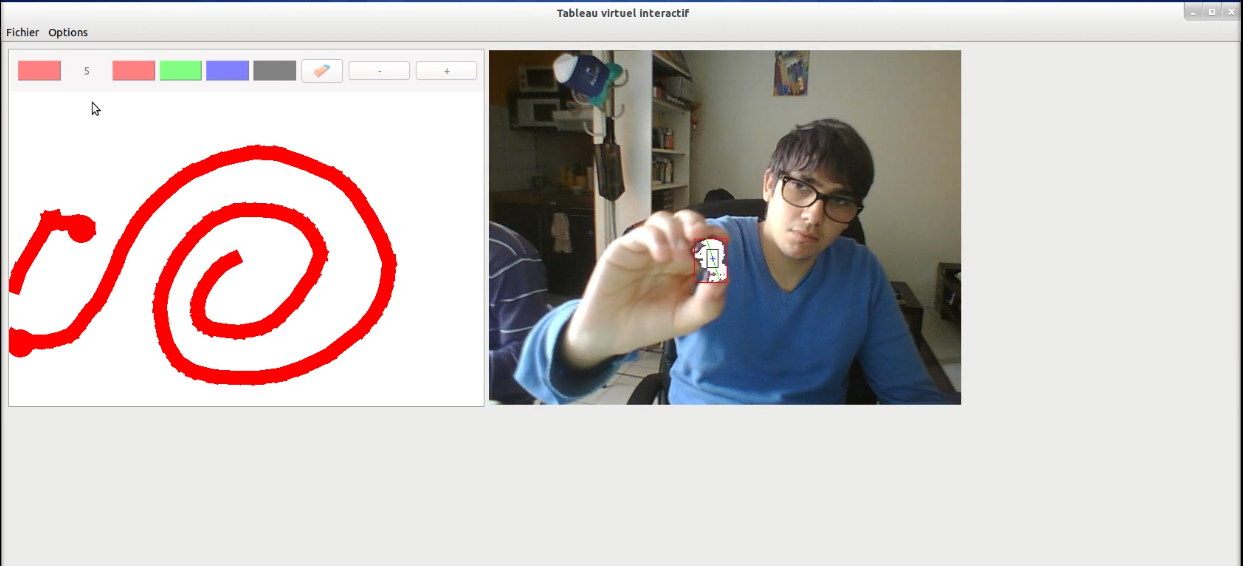
\includegraphics[scale=0.3]{../images/capture-intro.png}\\
			\caption{Aperçu de l'application}
			\label{Aperçu de l'application}
		\end{figure}
	\newpage
		\section{Contexte}
		% TODO
		Ce projet est réalisé dans le cadre des TER (Travaux d'Étude et de Recherche) de 1ère année de Master informatique à L'Université Montpellier 2. \\
		Le TER est un projet qui se déroule sur un semestre, généralement choisi par les étudiants parmi une liste de projets qui leurs sont proposés. \\Ce genre de projet apporte beaucoup aux étudiants. Il leur permet d'une part de travailler une longue période sur un seul et même sujet afin d'obtenir quelque chose de complet, d'abouti. \\D'autre part, le TER (comme son nom l'indique) apporte une bonne expérience dans le domaine de la recherche. En effet, un travail préalable doit être effectué sur l'existant (Est-ce que d'autres projets de ce genre existent? Si oui qu'ont-ils de différent?,...), mais également la faisabilité (Est-ce possible à faire? Quels algorithmes existent pour répondre à tel ou tel besoin?, ...). \\
		$$$$ \\
		La particularité de ce projet réside dans le fait que nous avons nous-même proposé ce sujet à un enseignant-chercheur.\\
		Nous avons décidé de proposer ce sujet pour diverses raisons, dont voici les pricipales:
		\begin{itemize}
			\item Tout d'abord, c'est un projet que nous avions en tête depuis plus d'un an, qui a donc eu le temps de murîr et d'être au niveau d'un TER.
			\item Deuxièmement, notre groupe vient de deux formations distinctes : \textbf{AIGLE}, formation orientée génie Logiciel ; et \textbf{IMAGINA}, spécialisée dans le jeu vidéo et l'image. Ce projet représentait une manière opportune de lier ces deux spécialités
			\item Enfin, ce projet était pour nous une bonne occasion de réaliser une application fonctionnelle et distribuable, et par conséquent nous permettre d'explorer une autre facette du développement d'applications : la mise en production.

		\end{itemize}	
	\chapter{Analyse et conception}
		\section{Étude de l'existant et faisabilité}
		\subsubsection{Faisabilité}
		% TODO : expliquer si ça nous parait possible 
		Notre groupe ayant lui-même proposé ce sujet, celui-ci s'accorde parfaitement à nos formations et spécialités. Le choix de ce sujet a donc été réalisé en fonction de nos expériences, savoir-faire et affinités.\\
Ce projet s'inscrivant dans le cadre d'un TER de notre formation, l'étude de la faisabilité n'incluera pas certains critères comme l'étude de marché, le contexte économique ou le besoin réel. 
Nous nous sommes concentrés notamment sur les compétences techniques et de gestion. Pour les parties financement et analyse des coûts, il va sans dire que nous ne disposions d'aucun financement et n'avons donc utilisé que des outils gratuits. \\

		\subsubsection{Existant}
		La vision par ordinateur et particulièrement le suivi d'objets, sont des domaines connus et pour lesquels il existe de nombreux travaux. Nous pouvons nous inspirer de certains de ces travaux afin de proposer des fonctionnalités plus pertinentes, éviter certains écueuils ou plus directement utiliser des outils existants comme la bibliothèque OpenCV.\\
			\begin{itemize}
				% TODO : détailler un peu plus l'existant
				\item Exemples dans le jeux vidéo : Kinect, Eye-toy, CamSpace (techniques pour l'IHM, par exemple, mouvements continus ou immobilité sur une zone).
				\item Exemples issus de thèses et de projets de recherche (techniques de programmations).
			\end{itemize}
			\begin{figure}[!h]
				\centering
				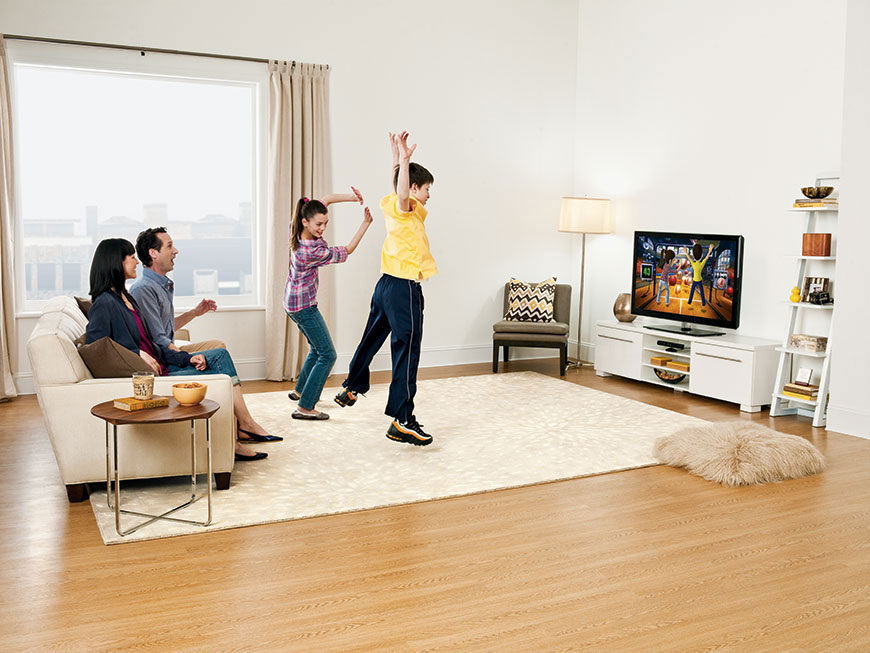
\includegraphics[scale=0.2]{../images/kinect_screen_lg.jpg}\\
				\caption{Exemple du Kinect}
				\label{Exemple du Kinect}
			\end{figure}
		\newpage
		\section{Gestion du projet}
			\subsection{Choix stratégiques}
			Lors de ce projet, nous avons distingué deux parties majeures.
			La première est une bibliothèque de suivi d'objets. La seconde, une application qui utilise cette bibliothèque pour réaliser un logiciel de dessin interactif. \\
			Ce choix présente plusieurs intérêts : \\
			\begin{itemize}
				\item{Premièrement, ce découpage permet de bien différencier les tâches. Le développement de la bibliothèque requiert des connaissances en traitement d'images pour tracer des couleurs/objets, appliquer des filtres, manipuler les images, etc. Ceci correspond parfaitement à la formation de deux membres du groupe(formation IMAGINA à l'UM2). 
				Le développement de l'application requiert quant à lui des connaissances en génie logiciel, pour l'architecture de l'application, en IHM, pour la réalisation de l'interface (logicielle et gestuelle), ou encore en réseau pour la mise en place de l'architecture client/serveur. 
				Ces différents points correspondent également parfaitement à la formation des deux autres membres du groupe. (Formation AIGLE à l'UM2). Ainsi, les tâches peuvent bien se répartir en fonction des connaissances et spécialités de chacun.} \\
				\item{Deuxièmement, l'intérêt de ce découpage est d'avoir deux projets à la fois complètement indépendants et complémentaires. En effet, la bibliothèque développée offre des fonctionnalités de suivi utilisables par n'importe quelle application.\\
				L'application se charge d'utiliser les fonctionnalités de traitement d'images de la bibliothèque en ajoutant une interface graphique, une couche réseau, une connexion aux webcams ou encore la récupération des images.
				La bibliothèque et l'application sont donc deux projets développés en parallèle et très modulaires. Notre application peut très bien utiliser une autre bibliothèque de traitement d'images, et la bibliothèque peut très bien être utilisée par d'autres applications qui offriraient des fonctionnalités totalement différentes de la nôtre.}
			\end{itemize}
			\newpage
			\subsection{Diagramme de Gantt}
			Étant donné que nous avons proposé notre propre sujet, la première étape a été de rédiger un cahier des charges pour définir ce que nous voulions faire et de quelle manière. \\
			Après ceci, nous avons commencé à effectuer des recherches du côté bibliothèque et application, pour savoir quels outils et techniques utiliser pour arriver à nos objectifs. 
		  Nous avons réservé plusieurs semaines pour effectuer des recherches et perfectionner notre idée du projet. Nous avons donc lu des articles de recherches sur des thématiques proches, effectuer des essais d'outils etc. Cette période d'analyse et de conception sert aussi à penser l'application en imaginant des cas d'utilisations (use cases) et en réalisant le diagramme de classes. \\
			
			Par la suite, la majeure partie du temps est réservée au développement en lui même, en prenant en compte la date de présentation du projet pour avoir une réalisation complète. \\  
			Bien entendu ces temps de développement s'accompagnent de réunions avec tout le groupe de projet ainsi que de travail pour lier nos deux sous-parties et les tester ensemble. \\
			Des documents comme le rapport ou la documentation furent produit au fur et à mesure du projet, pour rester en adéquation avec le travail accompli. Voici le rétroplanning qui illustre le déroulement chronologique du projet : \\
				\begin{figure}[!h]
					\centering
					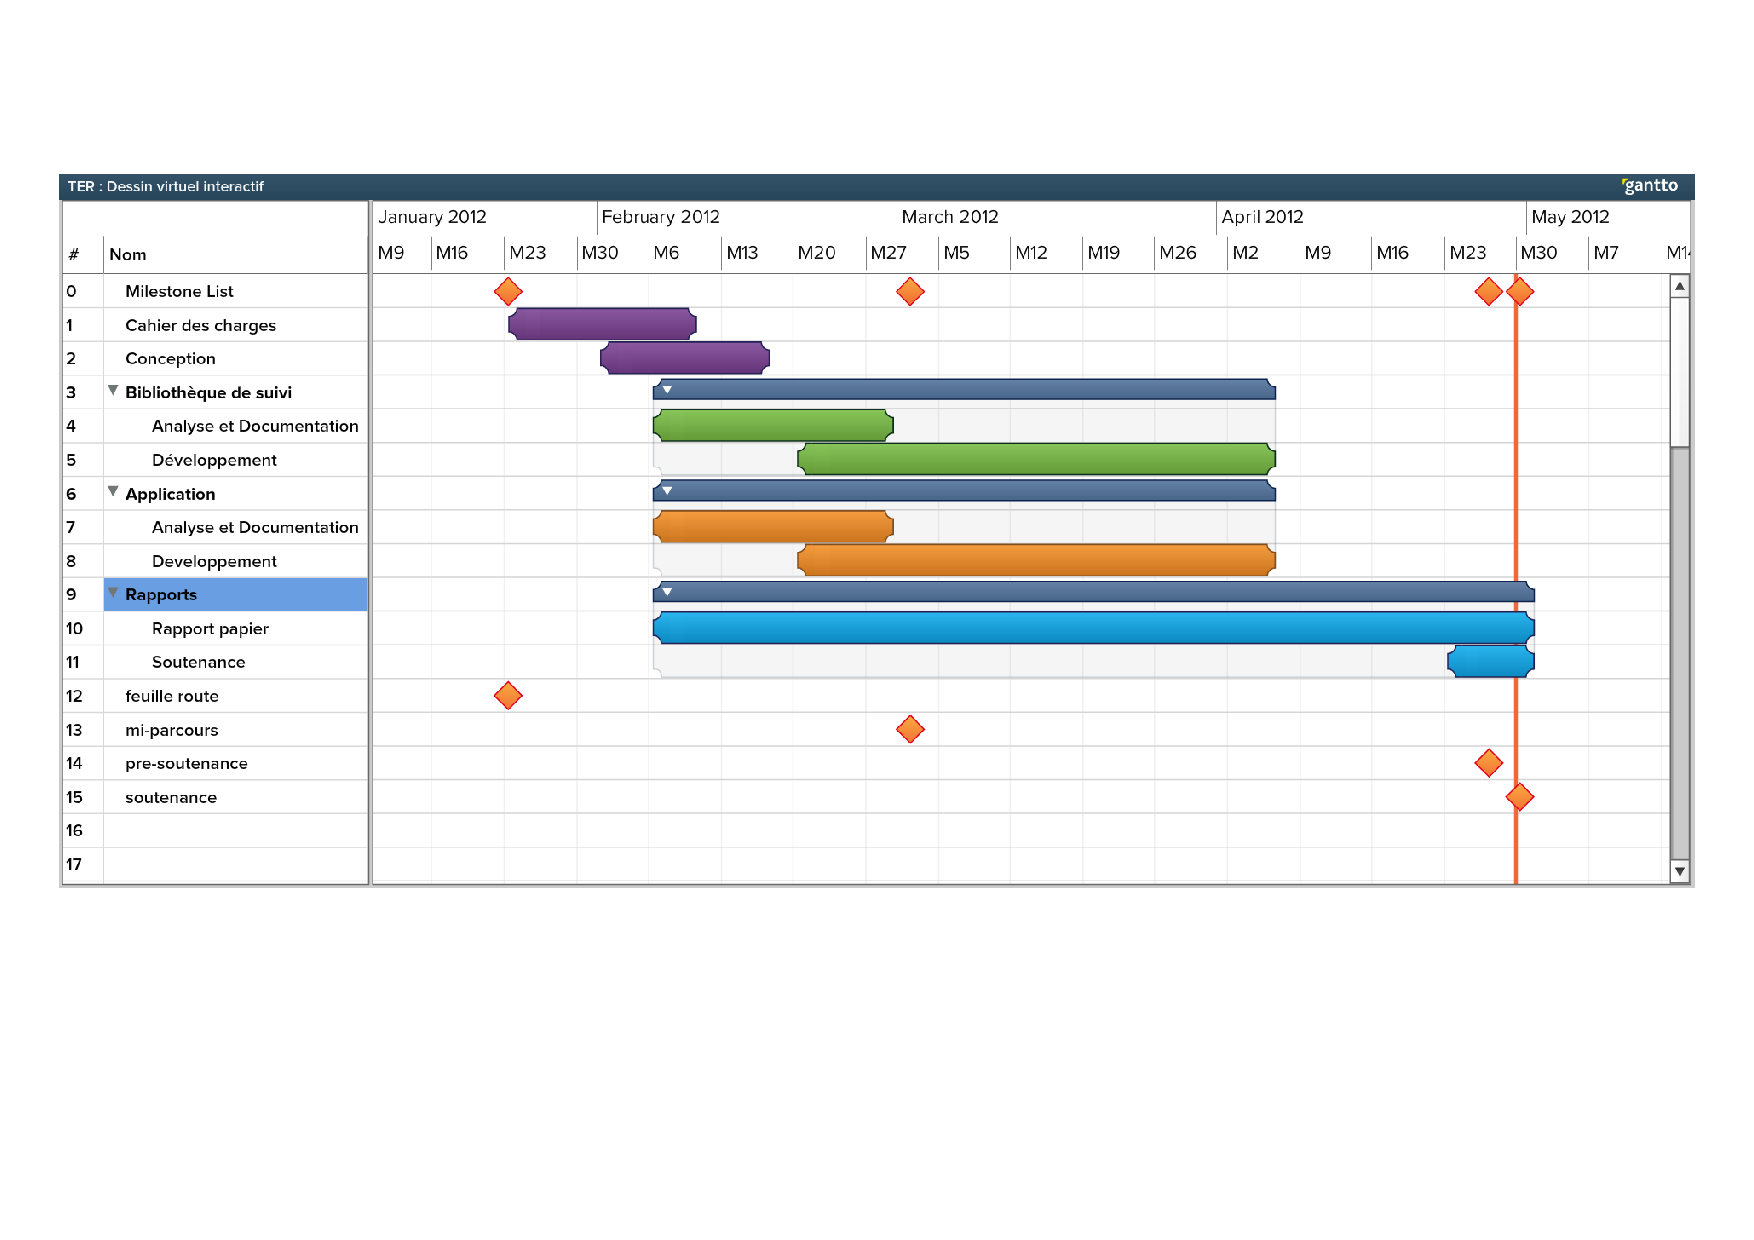
\includegraphics[scale=0.6]{../images/retro-planning.pdf}\\
					\caption{Rétroplanning}
					\label{Rétroplanning}
				\end{figure}
		\newpage
		\section{Outils utilisés}
		Durant la période de recherche et au cours du projet nous avons utilisé différent outils (au sens large) pour nous aider dans la réalisation. Nous les détaillons ici dans cette section. \\
		
			\subsubsection{Outils collaboratifs}
			\paragraph{}
			
\includegraphics[scale=1]{../logos/subversion-logo.png} 
			Subversion : Un gestionnaire de versions qui nous permettant de synchroniser notre travail, de partager le code source et de s'échanger quelques documents complexes (ce rapport par exemple).
			\paragraph{}
			
\includegraphics[scale=0.25]{../logos/Gobby-logo.png} 
			Gobby :
			Logiciel libre pour l'édition collaborative, qui permet de développer à distance sur le même document simultanément. \\

			\paragraph{} Bien sûr ces outils ne sont pas suffisants, nous avons donc fait des réunions régulières pour organiser le travail et décider des orientations. Par ailleurs, nous avons beaucoup échangé pour que tout le monde soit toujours au courant des différentes informations importantes.
			
			\subsubsection{Outils techniques}
			\subsubsection{Langages :}
			\paragraph{} Langage C pour la bibliothèque : ce langage est bien adapté à la réalisation d'une bibliothèque car il permet l'écriture de fonctions. Par ailleurs c'est un langage bien adapté au domaine du traitement de l'image car il est de bas niveau, et très rapide. De plus, nous avons utilisé des bibliothèques (OpenCV par exemple) qui ont été écrites initialement en C.
			\paragraph{} Langage C++ pour l'application : c'est un langage objet ce qui nous aidait pour la conception. Il est également très rapide et c'est un langage avec lequel nous sommes à l'aise et avons de l'expérience, ce qui nous évitait de devoir apprendre un nouveau langange, et par là de perdre un temps précieux.\\
			
			\subsubsection{Bibliothèques :}
			
\includegraphics[scale=0.15]{../logos/qt_logo.png}
			Qt : bibliothèque d'IHM (et bien plus) en C++, nous aide pour faire les interfaces graphiques, pour la partie réseau également où elle offre des abstractions agréables. \\
			\paragraph{}
			
\includegraphics[scale=1]{../logos/OpenCV_Logo.png}
			: bibliothèque de traitement de l'image, nous aide à exploiter la webcam et pour le traitement de l'image avec plusieurs fonctionnalités. \\
		
		\newpage
		\section{Analyse}
			\subsection{Cas d'utilisations}
				\begin{figure}[!h]
						\centering
						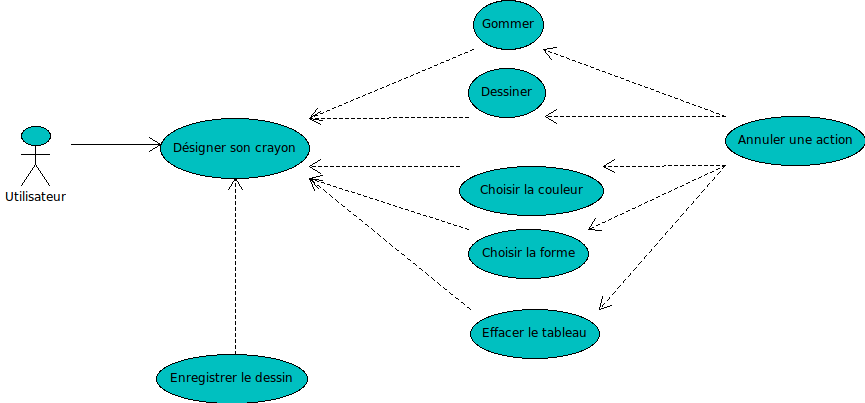
\includegraphics[scale=0.6]{../images/Dessin.png}\\
						\caption{Cas d'utilisation dessin}
						\label{Cas d'utilisation}
				\end{figure}
			\newpage
			\subsection{Diagrammes de séquences}
			Les diagrammes qui suivent expliquent le fonctionnement de l'application pour une utilisation locale, et une utilisation en réseau.
				\begin{figure}[!h]
						\centering
						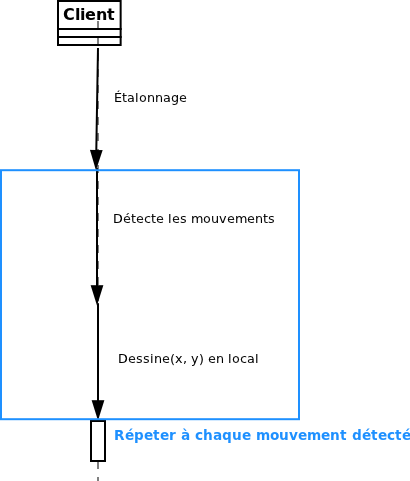
\includegraphics[scale=0.6]{../images/sequence_local.png}\\
						\caption{Diagramme de séquence local}
						\label{Diagramme de séquence local}
				\end{figure}
				On peut voir sur ce diagramme que le fonctionnement en local est assez basique. Dans un premier temps, l'utilisateur \textbf{étalonne} l'objet avec lequel il veut dessiner. Ensuite, lorsque l'utilisateur déplace l'objet en question, l'application \textbf{détecte} ce déplacement, et \textbf{dessine} à la nouvelle position de l'objet. Ce schéma de détection-dessin est répété jusqu'à fermeture de l'application. \\
				Ainsi, l'utilisateur verra se dessiner chacun des mouvements qu'il effectue avec son objet.

				\newpage
				\begin{figure}[!h]
						\centering
						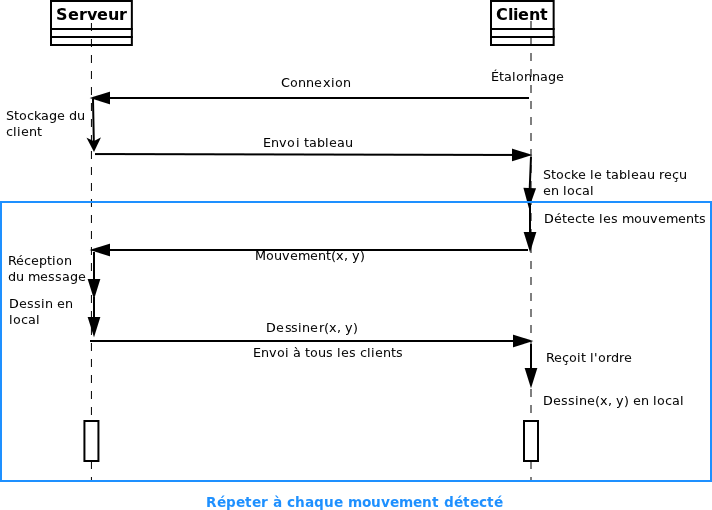
\includegraphics[scale=0.6]{../images/sequence_reseau.png}\\
						\caption{Diagramme de séquence réseau}
						\label{Diagramme de séquence réseau}
				\end{figure}
				En réseau, l'utilisation suit le même schéma, mais un autre acteur entre en jeu, le \textbf{serveur}. \\
				Comme pour une utilisation locale, l'utilisateur comment par \textbf{étalonner} l'objet à suivre. Puis, la connexion s'effectue auprès du serveur, qui va renvoyer le dessin courant au nouveau client. Une fois en possession du dessin, le client le stocke et peut rentrer dans la boucle de détection-dessin : \\
				Comme en local, l'application va \textbf{détecter} le mouvement de l'objet suivi. La nouvelle position est envoyée au serveur qui va dessiner sur son propre tableau, puis renvoyer à tous les clients l'ordre de \textbf{dessiner} à cette même position. Chaque client verra donc ce que les autres clients dessinent. \\
				Ainsi, l'utilisateur verra se dessiner chacun des mouvements qu'il effectue avec son objet, mais également ceux de tous les autres clients.
				\\ $$$$ \\
				On peut donc voir que pour l'utilisateur, le fonctionnement est identique qu'il dessine seul ou avec d'autres personnes :
				\begin{itemize}
					\item Il étalonne l'objet
					\item Il déplace l'objet
					\item l'objet dessine sur le tableau
				\end{itemize}
				
				Cependant, dans la pratique, le fonctionnement n'est pas le même. En réseau, chaque mouvement passe par le serveur qui se charge de faire le lien avec tous les clients de l'application.

			\newpage
			\subsection{Diagrammes de classes}
				La bibliothèque fonctionne grâce à une structure de données utilisée par deux fonctions enveloppes. \\
				Le curseur est représenté en mémoire sous la forme d'une strucure de données "Cursor". \\
				Cette structure de données est engendrée par la fonction "calibration" de la bibliothèque. Elle est ensuite utilisée par la fonction "track", qui permet la mise à jour des informations relatives au curseur par rapport à une image. \\
				\begin{figure}[!h]
						\centering
						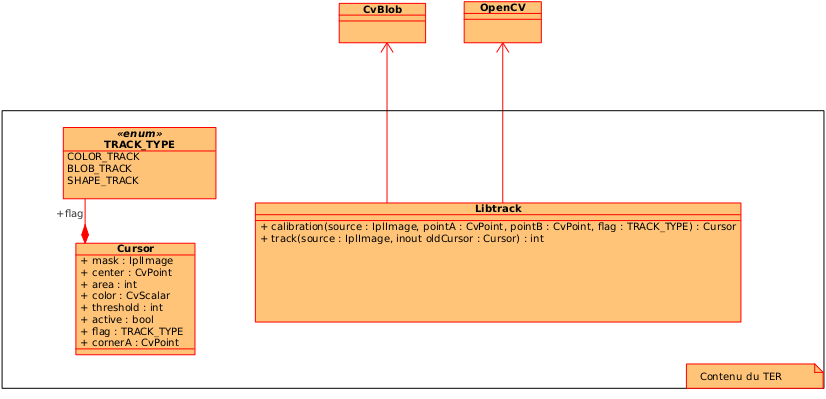
\includegraphics[scale=0.8]{../images/libtrack-uml.png}\\
						\caption{Architrecture de la bibliothèque}
						\label{Architrecture de la bibliothèque}
				\end{figure}

				La bibliothèque dépend de deux bibliothèques externes:
				\begin{itemize}
					\item OpenCV, Spécialisée dans le traitement des images
					\item CvBlob, bibliothèque issue d'OpenCV utlisée pour la recherche d'objet dans des images binaires
				\end{itemize}

				\newpage			
				Le diagramme qui suit vous présente l'architecture de notre application. \\
Avant de commencer l'application, nous avons décidé de passer un long moment sur la réflexion pour avoir une architecture solide et modulable.\\Nous avons dans un premier temps identifié les différents modules dont serait composée notre application et quel était précisément le ou les rôles de chacun. \\Ensuite, nous avons réfléchi à quel était le meilleur moyen pour que ces différents modules puissent communiquer en évitant toute redondance ou communication superflue. \\Une fois cette réflexion faite, nous avons dessiné le diagramme suivant : \\
				\begin{figure}[!h]
						\centering
						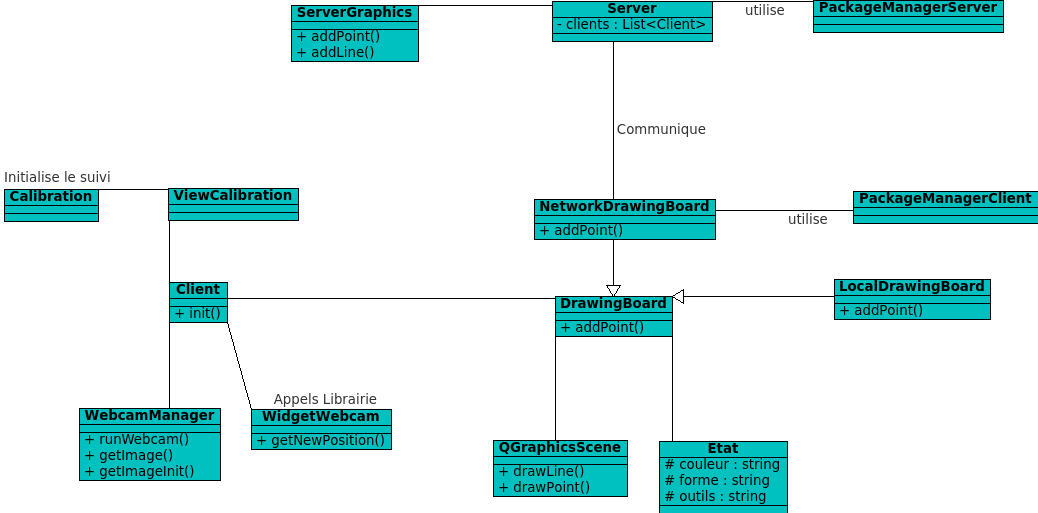
\includegraphics[scale=0.6]{../uml/classes.png}\\
						\caption{Diagramme de classe de l'application}
						\label{Diagramme de classe de l'application}
				\end{figure}
				
				On peut identifier quatre modules principaux : \\
				\begin{itemize}
					\item \textbf{Le module d'étalonnage} (Calibration et ViewCalibration). Ce module sert à tout ce qui touche à l'étalonnage de l'objet. Une fois qu'il est effectué, le module va appeler le module \textit{client} pour lui signaler que l'étalonnage est fait, et lui envoyer les informations qui correspondent (objet à suivre, type de suivi, dessin en local ou réseau, etc...)
					\item \textbf{Le module client} (Client). Ce module est le coeur de l'application, il a principalement deux rôles. Il va dans un premier temps construire toute l'interface graphique (tout ce qui est visuel) qui sera présentée à l'utilisateur. Ensuite, c'est ce module qui va assurer la communication entre tous les modules. Il est le seul intermédiaire entre les différents modules locaux.
					\item \textbf{Le module de dessin} (DrawingBoard, LocalDrawingBoard et NetworkDrawingBoard). Ce module a également deux rôles. Il va s'occuper de toute la partie dessin (Stocke la couleur et taille du pinceau, dessine les points, lignes, etc...). Aussi, pour une utilisation en réseau, c'est lui qui va se charger de communiquer avec l'application serveur.
					\item \textbf{Le module serveur} (Server, ServerGraphics). C'est ce module qui met en relation les différents client, et qui synchronise le dessin. Il reçoit les ordres de dessin, les stocke, et les renvoie à tous les autres clients.
				\end{itemize}
				\ \\
				La classe \textbf{WebcamManager} est la seule classe qui va communiquer avec le \textbf{matériel} (ici les webcams). Lorsque l'on veut une nouvelle image de la webcam, le module client va demander à WebcamManager la nouvelle image, et l'envoyer au module qui en a besoin. \\
				La classe \textbf{WidgetWebcam}, elle, est la seule classe qui va communiquer avec la \textbf{bibliothèque de suivi}. \\
				Les classes QGraphicsScene et Etat représentent respectivement le dessin et l'état actuel du pinceau. \\
				Les classes PackageManager* servent à assembler et désassembler les paquets qui transitent sur le réseau.
				\newpage
				\paragraph{Scénario :} \ \\
				Afin d'illustrer la modularité de notre application, on pourrait imaginer le scénario suivant :
				\begin{itemize}
					\item L'étalonnage s'effectue. Une fois terminé, le module d'étalonnage va prévenir le client, et lui donner les informations.
					\item Chaque X millisecondes, le client va interroger WebcamManager pour obtenir une nouvelle image.
					\item Le client va envoyer cette image à WidgetWebcam pour obtenir la nouvelle position. (Grâce à la bibliothèque de suivi)
					\item Le client va maintenant envoyer cette position à DrawingBoard qui va dessiner le nouveau point en fonction de la couleur la taille, etc...
				\end{itemize}
				On voit ici que chaque module rempli bien son rôle et assure le bon fonctionnement général de l'application.
				
				$$$$ \\
				Une fois cette phase de réflexion terminée, toute l'architecture de la bibliothèque, et de l'application était pensée et écrite. \\
				Nous pouvions alors débuter la phase de réalisation, programmer et imbriquer les différents modules, et s'attaquer aux problèmes plus techniques.

				
	
	\chapter{Réalisation}
		\section{Bibliothèque de suivi}
			Cette partie du développement a pour objectif de fournir un ensemble de fonctionnalités permettant la \textbf{reconnaissance} et le suivi d'un objet, que nous appellerons \textbf{Curseur}, à partir d'images. \\
			L'objectif est de développer notre propre \textbf{bibliothèque} pour d'une part avoir un outil remplissant précisément nos objectifs et d'autre part de faire un travail de recherche et développement dans le domaine du traitement de l'image (en particulier le suivi d'objets). \\
			Un certain nombre de bibliothèques existantes proposent des outils de reconnaissance de formes, de suivis de modèle ou d'évaluation de composantes connexes. Le travail consiste donc à tirer partie de ces bibliothèques en les associant de manière à proposer des méthodes efficaces et simples à utiliser. Cela implique une bonne connaissance des outils existants, de leur compréhension et de leur utilisation conjointe dans le but de concevoir notre propre bibliothèque. \\	
				\newpage
				\subsection{Aspect général}
				La structure générale de la bibliothèque est relativement simple à appréhender, ce qui permet une utilisation aisée sans connaissances particulières en traitement d'images.\\
				Comme expliqué dans la partie d'analyse, le fonctionnement de la bibliothèque de suivi repose sur l'utilisation d'une structure de données créée et manipulée respectivement par les deux fonctions d'étalonnage et de suivi. L'affinage de la recherche et le choix par l'utilisateur du type de suivi à réaliser passe par la manipulation d'une énumération, proposée par la bibliothèque. Aujourd'hui composée de 3 éléments correspondant chacun à un type de suivi particulier, cette énumération est amenée à s'agrandir avec l'ajout de nouvelles méthodes.
				\subsubsection{\textcolor{blue}{Étalonnage}} \paragraph{}
				Afin d'effectuer le suivi d'un objet (au sens large du terme) grâce à notre bibliothèque, il convient en premier lieu de faire appel à la fonction "calibration". Réalisant l'étalonnage, elle permet de créer et d'initialiser la struture de suivi, appelée "Cursor", contenant l'intégralité des informations qui vont permettre d'identifier l'objet et de réaliser sa localisation dans les images futures. C'est lors de cette étape que l'utilisateur doit préciser le type de suivi soubaité, par l'intermédiaire d'un simple paramètre.
					\paragraph{Fonctionnement}
					\begin{tabbing}
					\quad Du point de \=vue de l'utilisateur, une seule fonction permet de gérer la totalité de l'étalonnage, ce qui permet de simplifier\\ l'utilisation de notre bibliothèque : \\
					\>\begin{itshape}Cursor * calibration(IplImage * source, CvPoint A, CvPoint B, TYPE\_TRACK flag);\end{itshape}
					\end {tabbing}
					\quad Cette fonction, créant et initialisant la structure de suivi, n'est en réalité qu'une enveloppe faisant appel à une fonction différente selon le flag envoyé. Ces différences permettent de préparer la structure aux spécifités des fonctions de track et d'optimiser le suivi.
					\begin{tabbing}
					\quad Il suffit donc \=de lui passer l'image où se trouve l'objet, 2 points pour définir ses contours et enfin un flag déterminant la\\ méthode à employer, parmi les objet de l'énumération suivante : \\
\> \begin{itshape}enum TYPE\_TRACK \{TRACK\_COLOR, TRACK\_SHAPE, TRACK\_BLOB\};\end{itshape}
					\end{tabbing}
				\subsubsection{\textcolor{orange}{Suivi d'un objet}} \paragraph{}
				Une fois ces informations enregistrées, il est alors possible de faire appel autant de fois que nécessaire à la fonction "track" de suivi, afin mettre à jour la structure de données avec les modifications inhérantes au changement d'image.
						\paragraph{Fonctionnement}\paragraph{}
				\subsection{Détails techniques}
					\subsubsection{\textcolor{blue}{Fonctions d'étalonnage}}
						\paragraph{colorAverage} \paragraph{}
						Détails sur la fonction de colorAverage.
						\paragraph{mainColor} \paragraph{}
						Détails sur la fonction de recherche de couleur principale.
					\subsubsection{\textcolor{orange}{Fonctions de suivi}}
						\paragraph{Binarisation} \paragraph{}
							Détails sur la fonction de binarisation.
						\paragraph{blobFounding} \paragraph{}
						Détails sur la fonction de blobFounding.
						\paragraph{setNewCoord} \paragraph{}
						Détails sur la fonction de setNewCoord.
						\paragraph{shapeTrack} \paragraph{}
						Détails sur la fonction de reconnaissance par modèle.
						
		\section{Application}
	\paragraph{Application :\\}
L'application doit exploiter le plus efficacement possible la bibliothèque de reconnaissance. Nous voulons donc mettre en place un étalonnage de l'objet à suivre le plus précisément possible. Le projet doit ensuite être exploitable et utile, nous devons donc mettre en place un certain nombre d'outils tels que la possibilité de gommer, changer de forme, de couleur etc. 
Un module réseau est aussi prévu pour une utilisation concurrente et synchronisée. Et bien sûr la fonctionnalité clé de l'application est le tableau virtuel, qui devra donc être exploitable et le dessin devra être fidèle aux mouvements reconnus.
	\chapter{Résultats}
		Dans cette section nous allons présenter le résultat tangible de ce projet, en mettant en lumière l'utilisation de la bibiothèque de suivi au travers de l'application de dessin.
		\section{Client}
			Comme dit précedemment, l'application est composée de deux grandes parties, la \textbf{calibration} et le \textbf{dessin}.
			\subsection{Calibration}
				La calibration est la première étape dans l'utilisation du logiciel, cette section est étroitement liée à la fonction \textbf{calibration} de la bibliothèque. Cette section est composée de quatre interfaces, ou étapes, permettant l'\textbf{initialisation} d'un suivi d'objet. Chacune de ces étapes aura pour but d'obtenir les paramètres de la fonction calibration, mais aussi de permettre à l'utilisateur d'agir sur des attributs de réglage du suivi.
				\newpage
				Le premier écran de l'application est l'interface de sélection de webcam et de méthode de suivi.\\
				\begin{figure}[!h]
						\centering
						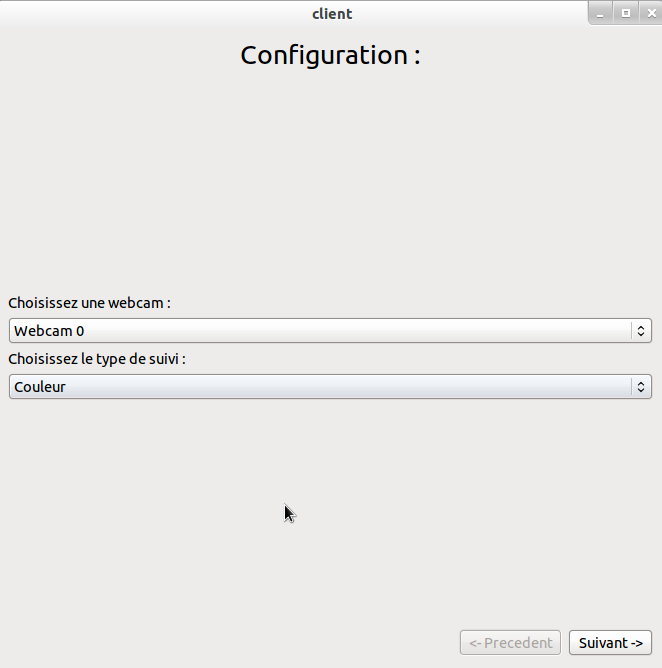
\includegraphics[scale=0.4]{../images/Capture6.png}\\
						\caption{Choix webcam/type track}
						\label{Choix webcam/type track}
				\end{figure}\\
				La première liste déroulante permet le choix de la webcam à utiliser pour la capture, la seconde la sélection de la méthode de track à parmi utiliser :
				\begin{itemize}
					\item Suivi par modèle
					\item Suivi par couleur
					\item Suivi par couleur + composantes connexes
				\end{itemize}

				Au niveau de la bibliothèque de suivi, ces listes servent à définir la sources des images servant au track, et à choisir le drapeau pour la fonction calibration.
				\newpage
				L'écran suivant permet quand à lui de sélectionner sur le retour image de la webcam l'objet à suivre, le curseur.\\
				\begin{figure}[!h]
						\centering
						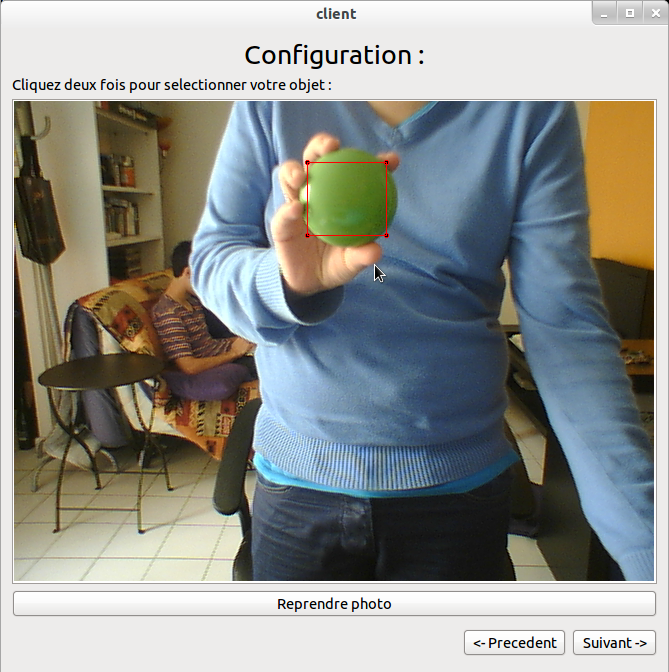
\includegraphics[scale=0.4]{../images/Capture1.png}\\
						\caption{Sélection du curseur}
						\label{Sélection du curseur}
				\end{figure}\\
				Il suffit pour cela, par clics sur l'image, de créer une boîte englobante autour du dit curseur.\\
				Cet écran sert à récuperer les coordonnées de la hit box nécessaire à l'isolement de l'objet pour le suivi par comparaison de modèle ou à l'extraction de la couleur et de l'aire de l'objet pour les suivis par couleur.
				\newpage
				\begin{figure}[!h]
						\centering
						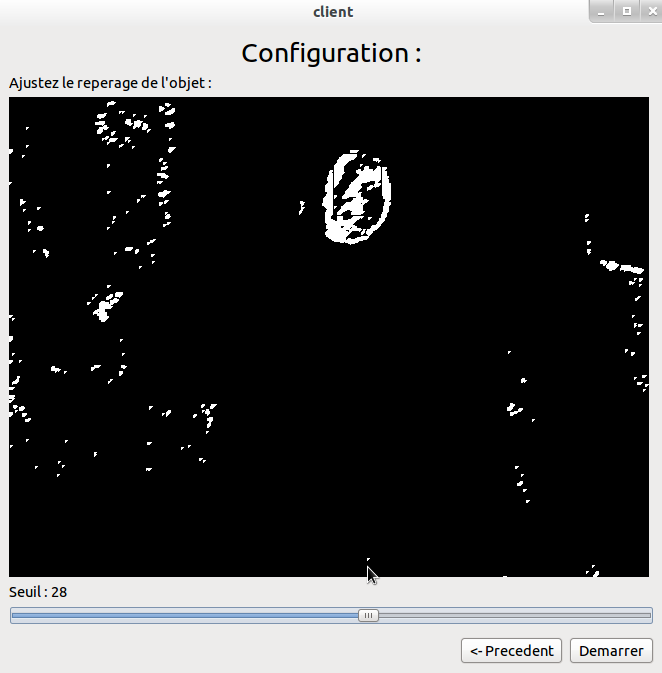
\includegraphics[scale=0.4]{../images/Capture2.png}\\
						\caption{Réglage du seuil}
						\label{Réglage du seuil}
				\end{figure}
				\newpage
				\begin{figure}[!h]
						\centering
						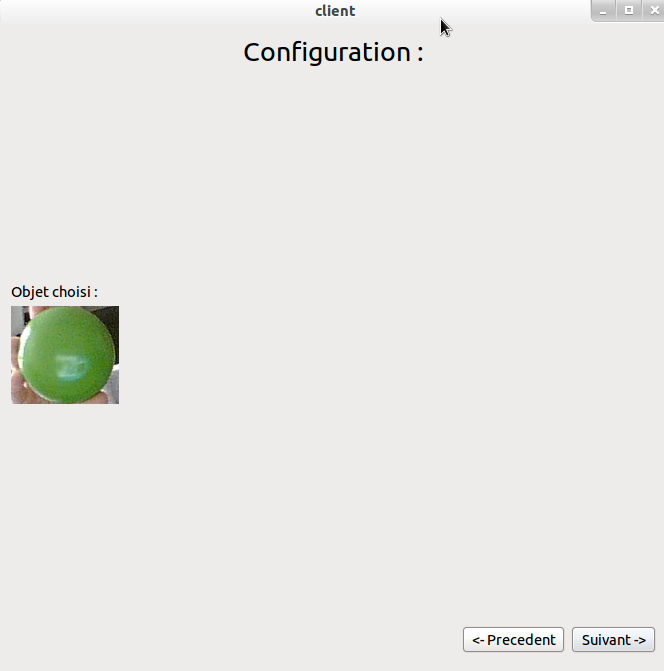
\includegraphics[scale=0.4]{../images/Capture7.png}\\
						\caption{Contrôle du modèle}
						\label{Contrôle du modèle}
				\end{figure}
				\newpage
				\begin{figure}[!h]
						\centering
						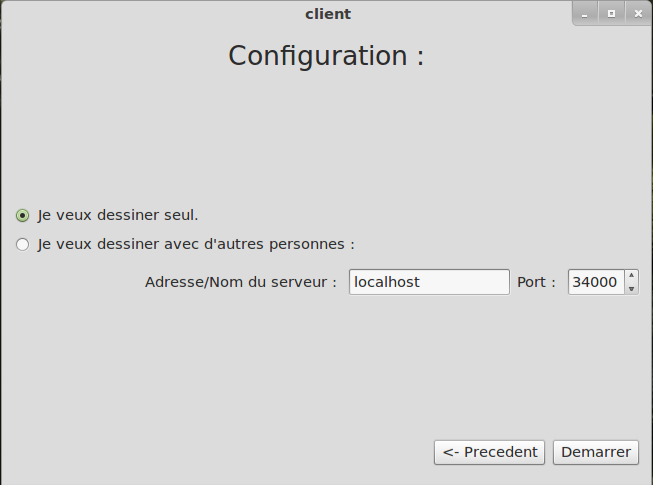
\includegraphics[scale=0.4]{../images/capture_choix.png}\\
						\caption{Sélecteur Local/Réseau}
						\label{Sélecteur Local/Réseau}
				\end{figure}
				\newpage
			\subsection{Dessin}
				\begin{figure}[!h]
						\centering
						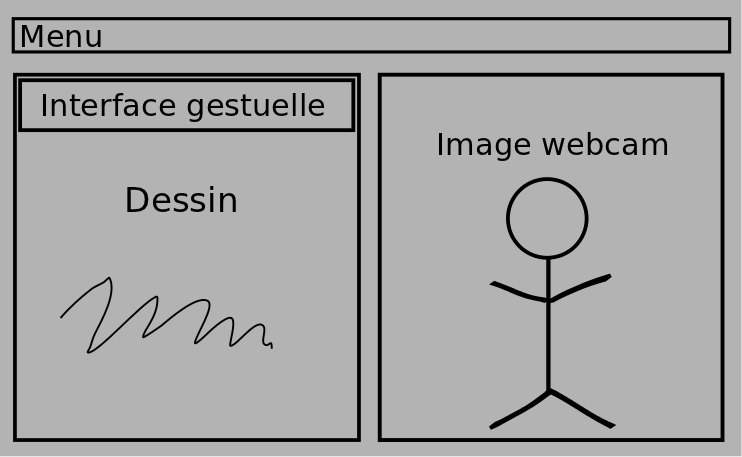
\includegraphics[scale=0.4]{../images/interface.png}\\
						\caption{Interface de dessin}
						\label{Interface de dessin}
				\end{figure}
				\newpage
				\begin{figure}[!h]
						\centering
						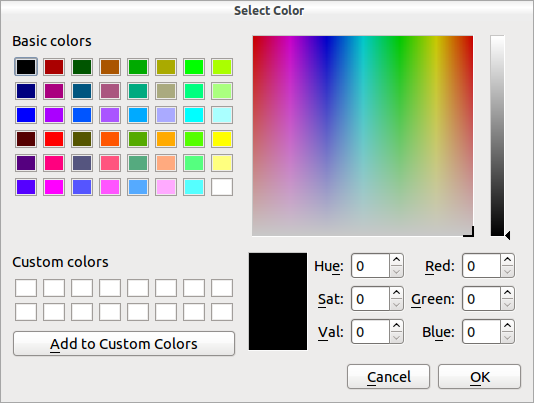
\includegraphics[scale=0.4]{../images/colorpicker.png}\\
						\caption{Selecteur de couleur}
						\label{Selecteur de couleur}
				\end{figure}
				\begin{figure}[!h]
						\centering
						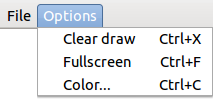
\includegraphics[scale=0.4]{../images/menu.png}\\
						\caption{Menu}
						\label{Menu}
				\end{figure}
				\begin{figure}[!h]
						\centering
						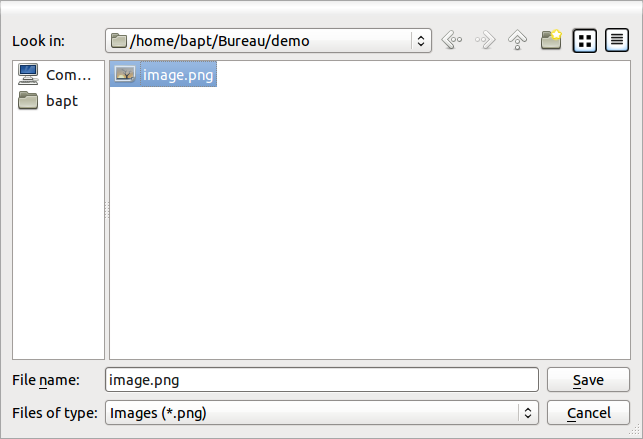
\includegraphics[scale=0.4]{../images/export.png}\\
						\caption{Export}
						\label{Export}
				\end{figure}
				\newpage
		\section{serveur}
		%Julien, Baptiste : y'a t'il assez de choses a dire pour en faire une partie? TODO
		
	
	\chapter{Conclusion}
		\section{Difficultés rencontrées}
		\section{Perspectives}
		\section{Conclusion}
	
	\chapter{Références}
	
	\part{Annexes}
	\appendix
		\chapter{Documentation de la bibliothèque}
		%
\includegraphics{../code-doc/refman.pdf}
\end{document}
